%%% Hlavní soubor. Zde se definují základní parametry a odkazuje se na ostatní části. %%%

%% Verze pro jednostranný tisk:
% Okraje: levý 40mm, pravý 25mm, horní a dolní 25mm
% (ale pozor, LaTeX si sám přidává 1in)
\documentclass[12pt,a4paper]{report}
\setlength\textwidth{145mm}
\setlength\textheight{247mm}
\setlength\oddsidemargin{15mm}
\setlength\evensidemargin{15mm}
\setlength\topmargin{0mm}
\setlength\headsep{0mm}
\setlength\headheight{0mm}
% \openright zařídí, aby následující text začínal na pravé straně knihy
\let\openright=\clearpage

%% Pokud tiskneme oboustranně:
% \documentclass[12pt,a4paper,twoside,openright]{report}
% \setlength\textwidth{145mm}
% \setlength\textheight{247mm}
% \setlength\oddsidemargin{14.2mm}
% \setlength\evensidemargin{0mm}
% \setlength\topmargin{0mm}
% \setlength\headsep{0mm}
% \setlength\headheight{0mm}
% \let\openright=\cleardoublepage

%% Vytváříme PDF/A-2u
\usepackage[a-2u]{pdfx}
\usepackage{listings}
\def\inline{\lstinline[basicstyle=\ttfamily,keywordstyle={}]}

%% Přepneme na českou sazbu a fonty Latin Modern
\usepackage[czech]{babel}
\usepackage{lmodern}
\usepackage[T1]{fontenc}
\usepackage{textcomp}

%% Použité kódování znaků: obvykle latin2, cp1250 nebo utf8:
\usepackage[utf8]{inputenc}

%%% Další užitečné balíčky (jsou součástí běžných distribucí LaTeXu)
\usepackage{amsmath}        % rozšíření pro sazbu matematiky
\usepackage{amsfonts}       % matematické fonty
\usepackage{amsthm}         % sazba vět, definic apod.
\usepackage{bbding}         % balíček s nejrůznějšími symboly
			    % (čtverečky, hvězdičky, tužtičky, nůžtičky, ...)
\usepackage{bm}             % tučné symboly (příkaz \bm)
\usepackage{graphicx}       % vkládání obrázků
\usepackage{fancyvrb}       % vylepšené prostředí pro strojové písmo
\usepackage{indentfirst}    % zavede odsazení 1. odstavce kapitoly
\usepackage{natbib}         % zajištuje možnost odkazovat na literaturu
			    % stylem AUTOR (ROK), resp. AUTOR [ČÍSLO]
\usepackage[nottoc]{tocbibind} % zajistí přidání seznamu literatury,
                            % obrázků a tabulek do obsahu
\usepackage{icomma}         % inteligetní čárka v matematickém módu
\usepackage{dcolumn}        % lepší zarovnání sloupců v tabulkách
\usepackage{booktabs}       % lepší vodorovné linky v tabulkách
\usepackage{paralist}       % lepší enumerate a itemize
\usepackage[usenames]{xcolor}  % barevná sazba

%%% Údaje o práci

\def\NazevSkoly{Gymnázium, Praha 6, Arabská 14}
% Název oboru včetně počátečního 'Obor'.
\def\NazevOboru{Obor programování}

% Název práce v jazyce práce (přesně podle zadání)
\def\NazevPrace{Informační systém pro školní jídelny}

% Název práce v angličtině
\def\NazevPraceEN{Information System for School Canteens}

% Jména autorů
% Abecedně podle příjmení
% TODO: Michail, je tvé křestní jméno napsáno dobře?
\def\AutorPrace{Tomáš~Černý, Martin~Havlíček, David~Koňařík, Michail~Spiridonov}

% Rok odevzdání
\def\RokOdevzdani{2019}
% Měsíc odevzdání
\def\MesicOdevzdani{Duben}

% Vedoucí práce: Jméno a příjmení s~tituly
\def\Vedouci{Mgr. Jan Lána}

% Nepovinné poděkování (vedoucímu práce, konzultantovi, tomu, kdo
% zapůjčil software, literaturu apod.)
\def\Podekovani{%
Poděkování.
}

% Abstrakt (doporučený rozsah cca 80-200 slov; nejedná se o zadání práce)
\def\Abstrakt{%
Cílem práce bylo vytvořit počítačový systém pro správu zařízení hromadného
stravování určený pro zaměstnance i strávníky. Systém řeší tvorbu jídelníčku,
správu seznamu strávníků a jejich kont a volbu jídel ze strany strávníků.
Pro tvorbu systému byly využity unikátní techniky a vlastní knihovny, které lze
dále využít pro další projekty.
}
\def\AbstraktEN{%
The goal of our project was to create a computer system for managing common
canteens aimed at both staff and diners. It deals with creating a menu, managing
a list of diners and their monetary accounts, and allows the diners to select
food in advance. To create this system we used unique techniques and developed
custom libraries, which can now be used for other projects.
}

% 3 až 5 klíčových slov (doporučeno), každé uzavřeno ve složených závorkách
\def\KlicovaSlova{%
{klíčová} {slova}
}
\def\KlicovaSlovaEN{%
{key} {words}
}

%% Balíček hyperref, kterým jdou vyrábět klikací odkazy v PDF,
%% ale hlavně ho používáme k uložení metadat do PDF (včetně obsahu).
%% Většinu nastavítek přednastaví balíček pdfx.
\hypersetup{unicode}
\hypersetup{breaklinks=true}

%% Definice různých užitečných maker (viz popis uvnitř souboru)
%%% Tento soubor obsahuje definice různých užitečných maker a prostředí %%%
%%% Další makra připisujte sem, ať nepřekáží v ostatních souborech.     %%%

%%% Drobné úpravy stylu

% Tato makra přesvědčují mírně ošklivým trikem LaTeX, aby hlavičky kapitol
% sázel příčetněji a nevynechával nad nimi spoustu místa. Směle ignorujte.
\makeatletter
\def\@makechapterhead#1{
  {\parindent \z@ \raggedright \normalfont
   \Huge\bfseries \thechapter. #1
   \par\nobreak
   \vskip 20\p@
}}
\def\@makeschapterhead#1{
  {\parindent \z@ \raggedright \normalfont
   \Huge\bfseries #1
   \par\nobreak
   \vskip 20\p@
}}
\makeatother

% Toto makro definuje kapitolu, která není očíslovaná, ale je uvedena v obsahu.
\def\chapwithtoc#1{
\chapter*{#1}
\addcontentsline{toc}{chapter}{#1}
}

% Trochu volnější nastavení dělení slov, než je default.
\lefthyphenmin=2
\righthyphenmin=2

% Zapne černé "slimáky" na koncích řádků, které přetekly, abychom si
% jich lépe všimli.
\overfullrule=1mm

%%% Makra pro definice, věty, tvrzení, příklady, ... (vyžaduje baliček amsthm)

\theoremstyle{plain}
\newtheorem{veta}{Věta}
\newtheorem{lemma}[veta]{Lemma}
\newtheorem{tvrz}[veta]{Tvrzení}

\theoremstyle{plain}
\newtheorem{definice}{Definice}

\theoremstyle{remark}
\newtheorem*{dusl}{Důsledek}
\newtheorem*{pozn}{Poznámka}
\newtheorem*{prikl}{Příklad}

%%% Prostředí pro důkazy

\newenvironment{dukaz}{
  \par\medskip\noindent
  \textit{Důkaz}.
}{
\newline
\rightline{$\square$}  % nebo \SquareCastShadowBottomRight z balíčku bbding
}

%%% Prostředí pro sazbu kódu, případně vstupu/výstupu počítačových
%%% programů. (Vyžaduje balíček fancyvrb -- fancy verbatim.)

\DefineVerbatimEnvironment{code}{Verbatim}{fontsize=\small, frame=single}

%%% Prostor reálných, resp. přirozených čísel
\newcommand{\R}{\mathbb{R}}
\newcommand{\N}{\mathbb{N}}

%%% Užitečné operátory pro statistiku a pravděpodobnost
\DeclareMathOperator{\pr}{\textsf{P}}
\DeclareMathOperator{\E}{\textsf{E}\,}
\DeclareMathOperator{\var}{\textrm{var}}
\DeclareMathOperator{\sd}{\textrm{sd}}

%%% Příkaz pro transpozici vektoru/matice
\newcommand{\T}[1]{#1^\top}

%%% Vychytávky pro matematiku
\newcommand{\goto}{\rightarrow}
\newcommand{\gotop}{\stackrel{P}{\longrightarrow}}
\newcommand{\maon}[1]{o(n^{#1})}
\newcommand{\abs}[1]{\left|{#1}\right|}
\newcommand{\dint}{\int_0^\tau\!\!\int_0^\tau}
\newcommand{\isqr}[1]{\frac{1}{\sqrt{#1}}}

%%% Vychytávky pro tabulky
\newcommand{\pulrad}[1]{\raisebox{1.5ex}[0pt]{#1}}
\newcommand{\mc}[1]{\multicolumn{1}{c}{#1}}



%% Titulní strana a různé povinné informační strany
\begin{document}
%%% Titulní strana práce a další povinné informační strany

%%% Titulní strana práce

\pagestyle{empty}
\hypersetup{pageanchor=false}

\begin{center}

{\LARGE\bfseries\NazevSkoly}

\vspace{-22mm}
\vfill

{\LARGE\NazevOboru}

\vfill

\centerline{\mbox{
\includegraphics[width=116mm]{../img/logo-ga.png}}}

\vspace{-8mm}
\vfill

{\bf\Large ROČNÍKOVÝ PROJEKT}

\vfill

% TODO: Upravit tak, aby všechna jména byla na jednom řádku
{\Large \AutorPrace}

\vspace{15mm}

{\LARGE\bfseries\NazevPrace}

% \vfill
% \Katedra
% \vfill

% \begin{tabular}{rl}

% Vedoucí bakalářské práce: & \Vedouci \\
% \noalign{\vspace{2mm}}

\vfill

\MesicOdevzdani \ \RokOdevzdani

\end{center}

\newpage

%%% Následuje vevázaný list -- kopie podepsaného "Zadání bakalářské práce".
%%% Toto zadání NENÍ součástí elektronické verze práce, nescanovat.

%%% Strana s čestným prohlášením k bakalářské práci

\openright
\hypersetup{pageanchor=true}
\pagestyle{plain}
\pagenumbering{roman}
\vglue 0pt plus 1fill

\noindent Prohlašuji, že jsem jediným autorem tohoto projektu, všechny citace
jsou řádně označené a všechna použitá literatura a další zdroje jsou v práci
uvedené.  Tímto dle zákona 121/2000 Sb. (tzv. Autorský zákon) ve znění
pozdějších předpisů uděluji bezúplatně škole Gymnázium, Praha 6, Arabská14
oprávnění k výkonu práva na rozmnožování díla (§ 13) a práva na sdělování díla
veřejnosti (§ 18) na dobu časově neomezenou a bez omezení územního rozsahu.

\vspace{10mm}

\hbox{\hbox to 0.5\hsize{%
V ........ dne ............
\hss}\hbox to 0.5\hsize{%
Tomáš Černý ............
\hss}}

\vspace{20mm}

\noindent Prohlašuji, že jsem jediným autorem tohoto projektu, všechny citace
jsou řádně označené a všechna použitá literatura a další zdroje jsou v práci
uvedené.  Tímto dle zákona 121/2000 Sb. (tzv. Autorský zákon) ve znění
pozdějších předpisů uděluji bezúplatně škole Gymnázium, Praha 6, Arabská14
oprávnění k výkonu práva na rozmnožování díla (§ 13) a práva na sdělování díla
veřejnosti (§ 18) na dobu časově neomezenou a bez omezení územního rozsahu.

\vspace{10mm}

\hbox{\hbox to 0.5\hsize{%
V ........ dne ............
\hss}\hbox to 0.5\hsize{%
Martin Havlíček ............
\hss}}

\vspace{20mm}
\noindent Prohlašuji, že jsem jediným autorem tohoto projektu, všechny citace
jsou řádně označené a všechna použitá literatura a další zdroje jsou v práci
uvedené.  Tímto dle zákona 121/2000 Sb. (tzv. Autorský zákon) ve znění
pozdějších předpisů uděluji bezúplatně škole Gymnázium, Praha 6, Arabská14
oprávnění k výkonu práva na rozmnožování díla (§ 13) a práva na sdělování díla
veřejnosti (§ 18) na dobu časově neomezenou a bez omezení územního rozsahu.

\vspace{10mm}

\hbox{\hbox to 0.5\hsize{%
V ........ dne ............
\hss}\hbox to 0.5\hsize{%
David Koňařík ............
\hss}}

\vspace{20mm}
\noindent Prohlašuji, že jsem jediným autorem tohoto projektu, všechny citace
jsou řádně označené a všechna použitá literatura a další zdroje jsou v práci
uvedené.  Tímto dle zákona 121/2000 Sb. (tzv. Autorský zákon) ve znění
pozdějších předpisů uděluji bezúplatně škole Gymnázium, Praha 6, Arabská14
oprávnění k výkonu práva na rozmnožování díla (§ 13) a práva na sdělování díla
veřejnosti (§ 18) na dobu časově neomezenou a bez omezení územního rozsahu.

\vspace{10mm}

\hbox{\hbox to 0.5\hsize{%
V ........ dne ............
\hss}\hbox to 0.5\hsize{%
Michail Spiridonov ............
\hss}}

\vspace{20mm}

% \newpage
%
% %%% Poděkování
%
% \openright
%
% \noindent
% \Podekovani

\newpage

%%% Povinná informační strana bakalářské práce

\openright

\vbox to 0.5\vsize{
\setlength\parindent{0mm}
\setlength\parskip{5mm}

Název práce:
\NazevPrace

Autoři:
\AutorPrace

% TODO: Je Lána vedoucí?
% Vedoucí práce:
% \Vedouci, \KatedraVedouciho

Abstrakt:
\Abstrakt

% Klíčová slova:
% \KlicovaSlova

\vss}\nobreak\vbox to 0.49\vsize{
\setlength\parindent{0mm}
\setlength\parskip{5mm}

% Opakování v angličtině.

Title:
\NazevPraceEN

Authors:
\AutorPrace

Abstract:
\AbstraktEN

\vss}

\newpage

\openright
\pagestyle{plain}
\pagenumbering{arabic}
\setcounter{page}{1}


%%% Strana s automaticky generovaným obsahem bakalářské práce

\tableofcontents

%%% Jednotlivé kapitoly práce jsou pro přehlednost uloženy v samostatných souborech
\chapter*{Úvod}
\addcontentsline{toc}{chapter}{Úvod}

Tato dokumentace a popsaný systém, Mocasys, jsme vytvořili jako skupinovou
ročníkovou práci pro předmět Programování ve 3. ročníku. Volbu tématu ovlivnilo
několik faktorů. Jeden z nich byla komplexita práce, která měla být adekvátní
týmu čtyř kompetentních programátorů. Dalším faktorem byla využitelnost
výsledného programu. Námi vytvořený systém pro jídelny může být, po malých
úpravách pro jednotlivé provozovny, použit jako náhrada existujícího komerčního
software.

Práci jsme pojali částečně i jako experiment v oblasti nástrojů a knihoven pro
tvorbu webových aplikací. Vytvořili jsme databázový framework DASCore, který
umožňuje jednoduše vytvářet databáze s ukládáním historie a ověřováním
uživatelských oprávnění na úrovni databáze. Dále jsme vytvořili knihovnu liwec
pro jazyk Scala, která umožňuje vytvářet grafická uživatelská rozhraní čistě v
tomto jazyce bez zbytečné komplexity.

\chapter*{Zadání}
\addcontentsline{toc}{chapter}{Zadání}

Cílem ročníkové práce bude vytvoření informačního systému pro školní jídelny (případně další hromadná stravovací zařízení).
Pracovníkům jídelny bude poskytovat možnost správy seznamu strávníků a jídel.
Strávníkům bude umožňovat volbu jídla na konkrétní dny.
Dle konzultací s potenciálními uživateli a dle analýzy existujících produktů bude zvolena další funkcionalita.
Součástí ročníkové práce bude rovněž hardwarové řešení pro výdej jídel pomocí identifikace fyzickými tokeny.

%%% Fiktivní kapitola s ukázkami sazby

\chapter{Architektura} \label{architektura}

% Nějaký pěkný obrázek

Mocasys se skládá z několika částí běžících na několika zařízeních.

\begin{itemize}
	\item \emph{\hyperref[backend]{Backend}} je samotná databáze systému. Je postavený na PostgreSQL.
	Narozdíl od konvenčních návrhů posílají další vrstvy systému SQL příkazy
	přímo do Backendu přes Middleend.
	
	\item \emph{\hyperref[middleend]{Middleend}} je vrstvou mezi ostatními částmi systému a Backendem.
	Řeší přihlašování a je dostupný jako webová REST služba.

	\item \emph{\hyperref[frontend]{Frontend}} je samotná webová aplikace. Je určena pro zaměstnance
	jídelny i strávníky a běží přímo v prohlížeči jako JavaScript.

	\item Výdejová čtečka je hardware určený k poloautomatickému výdeji
	jídla. Po přiložení identifikátoru ukáže obsluze zvolené menu.
\end{itemize}

\chapter{Backend} \label{backend}

Kód Backendu je rozdělen na dvě části, samotný Backend Mocasysu a
\\ \uv{DASCore}. DASCore poskytuje funkce pro řešení oprávnění přímo v
databázi a pro vytváření tzv. temporálních tabulek -- tabulek obsahujících i
historická data o každé změně.

Samotný Backend definuje tabulky systému a oprávnění nutná k jejich používání.
Tabulky jsou definovány standardní SQL syntaxí a pak jsou upraveny SQL funkcí.

Narozdíl od většiny systémů je vrstvám Mocasysu umožněn skoro přímý přístup k 
provádění SQL dotazů. Pro zajištění bezpečnosti bylo tak nutné implementovat
různá opatření přímo v databázi a využít tak pokročilé funkce PostgreSQL.

Při každém dotazu z Middleendu je vytvořeno spojení s databází a je spuštěna
funkce \texttt{session\_user\_set(user\_id, secret)}, kde \texttt{user\_id} je ID
uživatele získané z session tokenu a \texttt{secret} je klíč použitý k odhlášení
uživatele z daného databázového připojení a jeho navrácení do výchozího stavu.
Tato funkce, napsaná v jazyce Perl, uloží ID uživatele do globální proměnné pro
použití při ověřování práv.

Jednotlivé tabulky jsou pro potřeby uživatele databáze reprezentovány pomocí
\uv{views}, které mají nastavený atribut \texttt{security\_barrier}, což zakazuje
některé optimalizace a umožňuje tak použít \texttt{WHERE} klauzi k filtrování
tabulky dle oprávnění uživatele.

Omezení úprav je realizováno pomocí \texttt{INSTEAD OF} triggerů, které při
nedodržení podmínek zahlásí chybu a ukončí spojení.

Na verzované, temporální, tabulky je použito rozšíření PostgreSQL
\texttt{temporal\-\_tables} \citep[viz][]{TemporalTables} a pomocné funkce, které
k jedné tabulce vytvoří další pro ukládání historie a agregační view, které
zobrazí stav tabulky v globálně určeném čase.

Tato funkcionalita je obsažena ve funkcích, jejichž použití lze ukázat na
tabulce \texttt{food}:

\begin{code}
-- Vytvoří tabulku, ve které budou uložena data
CREATE TABLE IF NOT EXISTS food_current (
    id serial PRIMARY KEY,
    name text NOT NULL
);

-- Vytvoří tabulku pro ukládání historie a agregační view
SELECT version_table('food');

-- Stanoví nutná oprávnění k čtení a úpravám tabulky
SELECT dascore_setup_table('food',
    select_perm := $$ perm('food.select') $$,
    modify_perm := $$ perm('food.modify') $$);
\end{code}

\section{Databázové schéma}

Databázové schéma bylo navrženo obvyklými technikami jako jsou \uv{many-to-one} a 
\uv{many-to-many} vztahy a někdy i vztahem \uv{one-to-one}.
Bylo rozhodnuto, že se oddělí uživatel (tabulka \verb|users|),
strávník (tab. \verb|diners|) a osoba (tab. \verb|people|), 
což má několik důvodů. Ne každý uživatel musí být strávník.
Zároveň jedna osoba může mít více uživatelů, ale jeden uživatel
může mít k sobě přiřazeného pouze jednoho strávníka.
Příkladem budiž pracovník jídelny. Strávník může potenciálně být i třeba firma,
nebo jiný subjekt, takže je tak nechán prostor pro rozšíření.

Jak již bylo zmíněno, tabulky mají historii. Každá tabulka, kromě tabulky, která ukládá
data pro autentifikaci heslem, má suffix \emph{current} a párovou historickou tabulku,
která má suffix \emph{history}.

\paragraph{One to One}

\begin{itemize}
    \item users $\leftarrow$ user\_passwords\_data
    \item people $\leftarrow$ diners
\end{itemize}

\paragraph{One to Many}

\begin{itemize}
    \item people $\leftarrow$ users
    \item user\_mifare\_cards $\leftarrow$ users
    \item food $\leftarrow$ food\_assignments
    \item diner\_transactions $\leftarrow$ diners
\end{itemize}

\paragraph{Many to Many}

\begin{itemize}
    \item diners $\leftarrow$ food\_choice $\rightarrow$ food\_assignments
    \item users $\leftarrow$ user\_permissions $\rightarrow$ permissions
\end{itemize}

\noindent Na obrázku~\ref{dbSchema} můžeme vidět schéma s jednotlivými poli a jejich
datovými typy.

\begin{figure}
    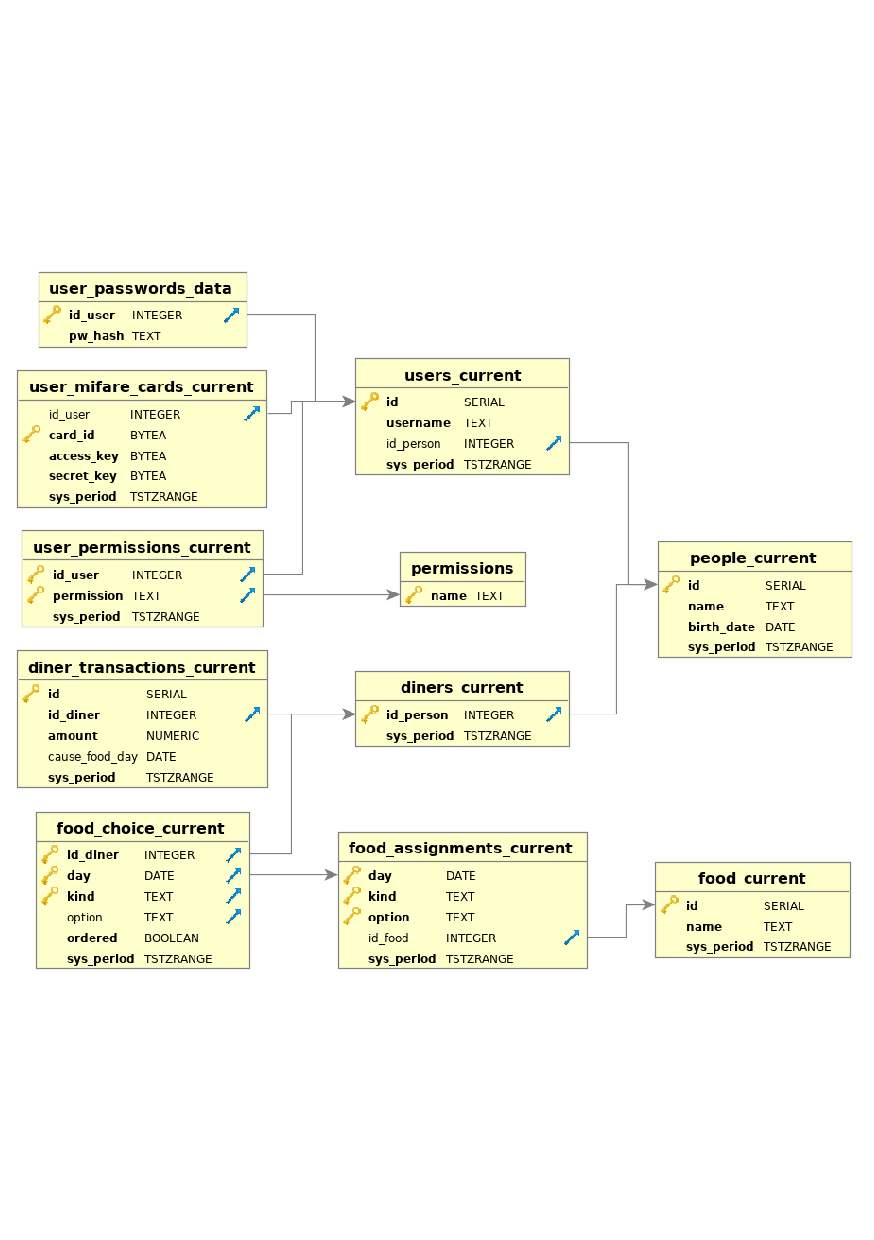
\includegraphics[width=140mm]{../img/db-schema}
    \caption{Databázové schéma. Vytvořeno programem DBVis.}
    \label{dbSchema}
\end{figure}

\chapter{Middleend} \label{middleend}


Middleend je napsán v jazyce Typescript pro Node.js za pomoci
RESTful frameworku Restify.
Ekosystém Node.js byl zvolen kvůli své škálovatelnosti a
rychlosti vývoje. Typescript, který je transpilován do JavaScriptu,
pak pomáhá omezit problémy spojené se slabě typovaným JavaScriptem
a přináší funkce v JavaScriptu nepřítomné nebo které by se
v JavaScriptu musely implementovat ručně či náročně.
Restify slouží jako užitečná abstrakce nad Node.js API.

Po spuštění se serverovému objektu Restify předají funkce pro parsování
příchozích žádostí, CORS mezivsrstva (z angl. Cross-Origin Resource Sharing).
Zmíněné funkce jsou přímo z frameworku Restify a přidružených NPM knihoven.
Před nasazením hlavního routeru je ještě přidána vlastní vrstva, která ověřuje
klientův \uv{session token}, o kterém si povíme v podsekci o autentifikaci.

Hlavní router skládá dohromady všechny endpointy, které mohou být umístěny
přímo na hlavní router, nebo mohou být součástí podřadných routerů.
Jeden takový podřadný router má na starosti přihlašování.
Je samozřejmě možné dávat endpointy přímo na serverový objekt,
ale tím bychom se zbavili jisté flexibility, a nemohli tak snadno
určit kořenovou cestu pro všechny endpointy.
Zároveň si každý router může určit, jakou relativní cestu budou mít
routery podřadné.

Veškerá komunikace s klinty je ve formátu JSON.

\section{Konfigurace}

Paramatry pro Middleend lze nastavit ze dvou míst. Z konfiguračního souboru,
jenž se nachází ve složce \verb|/config| a stanovením proměnné prostředí
(angl. Environment Variable) s názvem \verb|NODE_CONFIG|, jejíž hodnoty
mají prioritu nad konfiguračním souborem. Formát konfigurace je JSON:

\begin{code}
{
    "db": {
        ...
    },
    "server": {
        "port": 8000,
        ...
        "sessionTokenExpiresInMillis": 86400000,
        "rootPath": ""
    },
    "_desc": "Local development config."
}
\end{code}

Middleend používá dva Postgres účty. První (cesta \verb|db.middleend|) je určen například pro
ověřování a změnu hesel. Druhý (cesta \verb|db.qdb|) zajišťuje žádosti na endpoint \verb|/qdb|.
Druhý účet má práva pouze na pohledy na tabulky v db a jeho
permise dále omezují permise konkrétního uživatele. Objekty v polích \verb|db.*| mají
položky \verb|host|, \verb|port|, \verb|user|, \verb|password|, \verb|database|, \verb|max|.
Všechna kromě \verb|max| jsou na první pohled srozumitelná. \verb|Max| určuje nejvyšší možný počet klientů v poolu.

Chceme-li například změnit port aplikace, nastavíme \verb|NODE_CONFIG|
na řetězec \uv{\{"server": 9000\}}. Při spouštění v produkci je 
nutné nastavit \verb|NODE_ENV| na \newline \uv{production}.

\begin{table} \centering
\begin{tabular}{ l l l }
    {\textbf{Cesta}} & {\textbf{Typ}} & {\textbf{Popis}} \\
    \hline
    server.port & int & Port serveru \\
    server.origins & [string] & Povolené zdroje žádostí \\
    server.logRequests & bool & Logování obsahu žádostí \\
    server.sessionSecret & string & Tvorba klíčů pro session token \\
    server.sessionTokenExpiresInMillis & int & Doba platnosti session tokenu \\
    server.rootPath & string & Cesta hlavního routeru \\
    \hline
    server.authentication.password & boolean & Povolení přihlášení heslem \\
    server.authentication.reader & boolean & Povolení přihlášení kartou \\
\end{tabular}
\caption{Seznam všech používaných hodnot kromě databázového připojení}
\label{tb03:configKeys}
\end{table}

\section{Autentifikace}

Autentifikace může probíhat různými způsoby. Po úspěšné autentifikaci
uživatele nebo například čtečky, obdrží klient \uv{session token}, který
použije pro další žádosti. Posílá se v HTTP hlavičce \verb|Authorization|
ve formátu \uv{Token <hodnota>}. Klient také obdrží jeho dobu platnosti
v milisekundách od času autentifikace. Důvod pro autentifikaci hlavičkou
místo běžných cookies je, že tak jednoduše zabráníme XSS (angl. Cross-site scriping).

Session token má následující podobu: \newline
\verb|<iv>.<tělo>.<timestamp vytvoření>.<hmac>|. \verb|Iv| je inicializační vektor \citep[viz][]{TechopediaIV}.
Algoritmus pro vytvoření byl převzán z
knihovny node-client-sessions společnosti Mozilla \citep[viz][]{MozillaSession}.
Funguje tak, že si vytvoříme klíč pro šifrování dat, která jsou ve formátu JSON,
a klíč pro podepsání konečné zprávy. Klíče vytvoříme z náhodného řetězce (\uv{session secret}) pomocí funkce HMAC.
Session secret musí zůstat tajný, jinak by si útočník mohl sám podepsat session tokeny.
Symetricky zašifrujeme data, přičemž přidáme inicializační vektor.
Poskládáme jednotlivé části dohromady a spočítáme z nich HMAC
(angl. Hash Message Authentication Code), jehož hodnotu přidáme na konec celého tokenu.
HMAC slouží jako ověření tokenu, pouze Middleend je schopen ji vytvořit \citep[viz][]{SecSA}.
Inicializační vektor, zašifrovaná data, HMAC hodnotu závěrečně zaenkódujeme do Base64 \citep[viz][]{RFC4649}.

Aby byl předložený session token platný, musí splňovat několik podmínek.
Nesmí být starý, tj. $t_v + t_e \geq t$,
kde $t$ je nynější čas, $t_v$ je čas vytvoření a $t_e$ je čas, za který se token stane neplatným.
Po dešifrování si spočítáme znovu HMAC, a ten se musí rovnat HMAC hodnotě z tokenu.
Poslední podmínkou je úspěšné parsování dešifrovaných JSON dat.

\subsection{Autentifikace heslem}

Pro solení a hashování hesel využívá Middleend algoritmus scrypt, který
je pro Node.js dostupný jako NPM balíček stejného jména \citep[viz][]{NodeScrypt}.
V porovnání s jinými kryptografickými algoritmy používanými pro zabezpečení hesel,
jako je pbkdf2 nebo bcrypt, má pár výhod.
Používá exponenciální čas a paměť, takže hardware optimalizovaný pro jeho výpočet
není natolik účinný, jako je hardware například pro pbkdf2 \citep[viz][]{MediumScrypt}.
V praxi je ale pbkdf2 s mnoha iteracemi účinný a používáný.

\begin{table}[htb]\centering
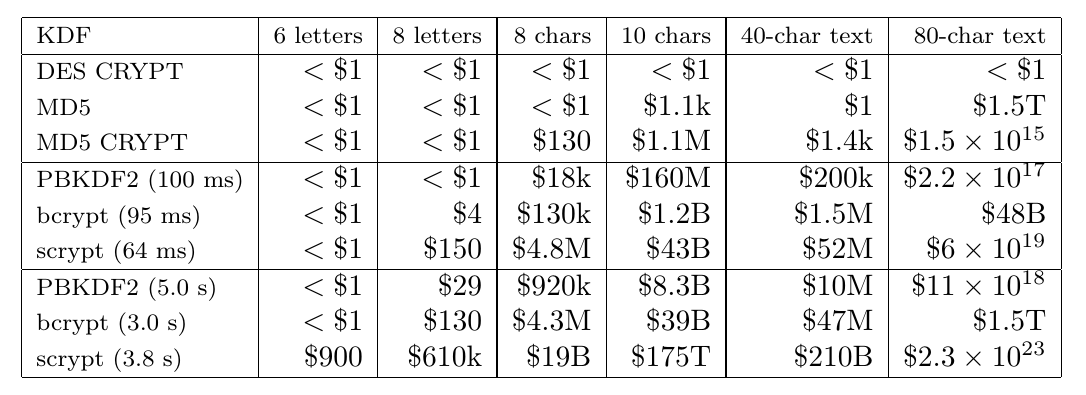
\includegraphics[width=140mm]{../img/crypto-funcs}
\textit{Časová hodnota v závorkách algoritmů určuje jejich náročnost.}
\caption{Odhadovaná cena hardwaru k prolomení hesla za 1 rok. \citep[viz][]{ScryptTable}}
\label{passwordCrackingCost}
\end{table}

Ceny hardwaru v tabulce~\ref{passwordCrackingCost} nebudou odpovídat dnešnímu stavu,
protože se výkon i cena hwardwaru od roku 2009, kdy byla tabulka vytvořena, změnily.
Každopádně je rozumné se domnívat, že crackování funkce scrypt je stále
nejdražší i dnes.

\section{Tunelování Postgresu pro Frontend}

Připojení k databázi je zprostředkováno NPM modulem \verb|pg| \citep[viz][]{NodePg}.
Ten umožňuje asynchronní přístup, předpřipravené žádosti a \uv{poolování}
(tj. máme \uv{pool} klientů, které si půjčujeme a vracíme je, jakmile je nepotřebujeme).

Jakmile je uživatel autentifikován platným session tokenem, je půjčen klient k databázi.
Dále se pošle databázi žádost, která zavolá backendovou funkci
\verb|session_user_set(user_id, secret)|, kde
\verb|user_id| je identifikátor uživatele a \verb|secret| je náhodný řetězec, který
potřebujeme pro odhlášení po spuštění uživatelského SQL.
Tím se určí uživatel a jeho permise.
Poté se spustí uživatelské SQL a odpověď se pošle uživateli.
Před posláním je ještě zpracována a některé části odpovědi z databáze jsou
vynechány, nebo přetransformovány.
V posledním kroku je uživatel odhlášen backendovou funkcí \verb|session_logout(secret)|,
kde \verb|secret| je náhodný řetězec, který jsme si vygenerovali při přihlášení.

\section{Transformace Postgres odpovědi}

Transformaci zajišťuje třída \verb|MiddleResponse|, která přijme původní odpověď databáze.
Odpověď databáze obsahuje proměnnou \verb|field| obsahující pole definic sloupců vrácených
z databáze.

\begin{code}
"fields": [
    {
        "name": "id",
        "tableID": 17249,
        "columnID": 1,
        "dataTypeID": 23,
        "dataTypeSize": 4,
        "dataTypeModifier": -1,
        "format": "text"
    },
    ...
]
\end{code}

V definici každého typu se chceme zbavit \verb|tableID|, \verb|columnID|, \verb|dataTypeID| a
nahradit je jmény, aby mohl Frontend data snadněji parsovat, čehož docílíme dotázáním se databáze.
Můžeme si všimnout, že v původní odpovědi už dostaneme název sloupce, jehož název může být
i agregační sloupec nebo sloupec přejmenovaný apod.
Dotazování z výkonostních důvodů provedeme při spuštění Middleendu.
SQL dotazy vypadají následovně:

\begin{code}
SELECT oid, typname FROM pg_type; -- id datových typů -> jména dt.
SELECT oid, relname FROM pg_class; -- id tabulek -> jména tabulek
\end{code}

Druhý SQL dotaz vrátí více než tabulky. Počet řádků je však dostatečně malý a nepotřebuje
moc paměťi navíc \citep[viz][]{PgType}, \citep[viz][]{PgClass}.

Odpovědi si uložíme do JavaScript objektu, který mapuje číselné identifikátory na řetězce.
JavaScript ale neumožňuje používat čísla jako klíče, tudíž si je převedeme při ukládání a
čtení na řetězec.

Konečná odpověď z Middleendu může vypadat následovně:

\begin{code}
{
    "rows": [
        [1, "Adam", "Warlock", "2014-04-08T22:00:00.000Z"],
        [2, "Harry", "Potter", "1990-07-31T22:00:00.000Z"]
    ],
    "rowCount": 2,
    "fields": [
        {
            "tableName": "wizards",
            "columnName": "id",
            "dataTypeName": "int4",
            "dataTypeSize": 4,
            "dataTypeModifier": -1,
            "format": "text"
        },
        ....
    ]
}
\end{code}

\chapter{Frontend} \label{frontend}


Webové rozhraní Mocasysu je napsané jako SPA (z angl. Single Page Application)
v jazyce Scala s využitím kompilátoru Scala.js. Byl vybudován na vlastním
frameworku \uv{liwec}, který je sám postaven na JavaScript knihovně domvm
\citep[viz][]{DomVm}. Využívá přístup \uv{virtual DOM} známý například z
knihoven React a Vue.

\section{Liwec}

Liwec dělí aplikaci na tzv. komponenty, někdy nazývané widgety či zobrazení,
které reprezentují jednotlivé soběstačné části grafického rozhraní. Komponenty
jsou třídy dědící abstraktní třídu \texttt{Component}. Při změně jakéhokoliv
atributu komponenty je spuštěna funcke \texttt{render()}, její výsledek
porovnán s aktuálním stavem a změny vykresleny. Hlídání změn využívá
\texttt{Proxy} \citep[viz][][MdnJsProxy], funkcionalitu JavaScriptu, která
umožňuje obalit objekt a při jakémkoliv přísupu k objektu zavolat handler
funkci.

Liwec umožňuje programovat aplikace výhradně ve Scale. Obsahuje DSL (z angl.
Domain Specific Language) pro tvorbu HTML a CSS, které využívají flexibilitu
Scaly, což dovoluje mít pro jednu komponentu pouze jeden soubor bez nutnosti
vkládat další jazyky jako text.

HTML tagy jsou reprezentovány objekty, což dovoluje například vytvářet
\uv{pseudo-komponenty} -- funkce, které dle daných parametrů vrátí HTML tag.
Tyto funkce zabírají méně paměti než plné komponenty, nemohou ale udržovat
vnitřní stav pomocí hlídaných atributů, plní tak jinou roli než plné komponenty.

U CSS bývá problémem \uv{přelévání} stylů z jedné komponenty do druhé kvůli příliš
širokým selektorům či sdíleným jménům tříd. Tento problém je někdy řešen
komplikovanými vývojovými metodologiemi, liwec však implementuje \uv{scoped CSS},
koncept převzatý z Vue. Každému DOM elementu je přidán atribut, který unikatně
identifikuje komponentu, které je součástí. Ke každé části každého CSS selektoru
je pak přidána ekvivalentní podmínka.

CSS styly komponent jsou při kompilaci převedeny makrem na textovou reprezentaci
a uloženy do souborů, poté sloučeny externím skriptem. Výsledná aplikace tak
nemusí obsahovat kód na generování CSS.

% TODO: Make this a floating figure
\begin{code}
class Counter(var i: Int = 1) extends Component {
    def render() = scoped(div(
            button("Increment",
                   onClick := { _ => i += 1 }),
            div(s"Counted to \$i")
    ))
    cssScoped { import liwec.cssDsl._
        e.div (
            color := "crimson",
            fontSize := "20pt",
        )
    }
}
\end{code}

\subsection{Interní struktura}

Liwec je kompilován nástrojem SBT. Jeho tzv. projekt je rozdělen na několik dílčích projektů:

\begin{itemize}
	\item \emph{macros} obsahuje makra využívaná v DSL liwecu, konkrétně
	\texttt{scoped} pro úpravu HTML pro \uv{scoped CSS}. Dále pak
	\texttt{css} a \texttt{cssScoped}, makra pro zpracování CSS DSL.

	\item \emph{htmlCodegen} a \emph{cssCodegen} jsou programy, které ze
	stránek MDN získají data ve strukturované formě a vytvoří pak podle
	nich třídy a funkce, které pak jsou součástí DSL.

	\item \emph{liwec} obsahuje samotný kód obsažený v zkompilovaném výstupu,
	mimo jiné typy pro DSL, reprezentaci knihovny \texttt{domvm} ve Scale
	(tzv. \uv{binding}) a kód pro routování stránek dle URL.
\end{itemize}

\subsection{HTML DSL}

Vytváření HTML komponent pomocí DSL, sady prvků jazyka tvořících vnořený
\uv{jazyk}, je jednou z definujících vlastností liwecu. Tento přístup je
inspirován mimo jiné JavaScript knihovnou Mithril \citep[viz][]{MithrilJs} a
Scala knihovnou ScalaTags \citep[viz][]{ScalaTags}.

DSL je implementováno pomocí různých funkcí Scaly, několik z nich exklusivních
tomuto jazyku. Tagy jsou reprezentovány statickými objekty (konkrétně
\texttt{lazy val}), které lze volat jako funcke akceptující libovolné množství
argumentů a vracející objekt \texttt{Element\-VNode} z knihovny \texttt{domvm}.
Tyto objekty lze chápat jako \uv{typesafe} wrappery funkce \texttt{el} z
\texttt{domvm}.

Argumenty tagů jsou instance \uv{vlastnosti} (angl. trait)
\texttt{VNode\-Applicable[T]}, kde \texttt{T} je typ elementů, na které lze tuto
instanci použít. Každá instance \texttt{VNode\-Applicable} má metodu
\texttt{applyTo(vn: T): Unit}, která zmutuje předaný objekt. Instancí
\texttt{VNode\-Applicable} jsou mimo jiné objekty reprezentující atributy tagů a
jejich hodnoty a komponenty. Pomocí tzv. implicitních tříd lze pak jako
\texttt{VNode\-Applicable} brát i například řetězce, další elementy a vybrané
monády (\texttt{Seq} a \texttt{Option}), pokud obsahují další
\texttt{VNode\-Applicable}.

Atributy tagů jsou objekty, které po použití operátoru \texttt{:=} vrátí objekt
reprezentující název atributu i jeho hodnotu. Tento objekt je instancí
\texttt{VNode\-Applicable}, takže je možné jej použít jako argument tagů.

\subsection{CSS DSL}

Popis CSS pravidel v liwecu využívá objektů a vlastních operátorů k vytvoření
AST (z angl. Abstract Syntax Tree, syntaktický strom). CSS selektory jsou
reprezentovány instancemi \texttt{Selector}, které jsou vytvářeny primárně
pomocí globálních \uv{dynamických objektů}. Díky funkci Scaly je
\texttt{c.className} přetransformováno na \texttt{c.selectDynamic("className")},
což je v liwecu funkce vracející selektor pro CSS třídu nazvanou
\texttt{className}. Komplexní selektory lze pak vytvářet pomocí vlastních
operátorů vlastnosti \texttt{Selector}.

Selektor je možné buď zavolat jako funkci přímo, nebo zavolat jeho metodu
\texttt{->}. Obě funkce berou libovolné množství parametrů: samotné CSS
vlastnosti a další pravidla. Takto vzniklé pravidlo je pak zpracováno makry
\texttt{css} a \texttt{cssScoped}.

\section{Tabulky a formuláře}

Velkou část Frontendu tvoří rutinní tabulky a formuláře, které skoro přesně
odpovídají SQL tabulkám. Proto byly vytvořeny obecné třídy a funkce pro
vytváření těchto konstruktů.

Framework tabulek se skládá ze dvou vrstev. Nižší umožňuje z jakéhokoliv seznamu
a specifických objektů sloupců vytvořit tabulku, druhá se pak zaměřuje na
vytváření tabulek z libovolného SQL dotazu.

Framework formulářů je navržen vesměs dynamicky. Jádrem každého formuláře je
\texttt{Map[String, Any]}, slovník z řetězce na libovolný datový typ. Tento
přístup sice znatelně ztěžuje ověřování správnosti kódu při kompilaci, výsledný
kód je ale velmi krátký a framework nevyžaduje k funkčnosti žádná komplexní
makra.

\section{Hlavní menu}

Menu můžeme reprezentovat rekurzivně dvojící tříd \verb|MenuItem|
a \verb|SubMenu|. Obě tyto třídy dědí z traitu (interface v Javě) \verb|MenuNode|,
což zjednodušuje psaní algoritmů, jenž využívají instance
těchto tříd. Limitujeme tak počet případů.
\verb|MenuItem| uchovává text odkazu a funkci, která se zavolá
při kliknutí na odkaz.
\verb|SubMenu| si uchovává \verb|MenuItem|
seznam \verb|MenuNode|, abychom mohli menu reprezentovat rekurzivně.

\begin{code}
trait MenuNode
class MenuItem(value: String, action: Event => Unit) extends MenuNode
class SubMenu(item: MenuItem, children: Seq[MenuNode]) extends MenuNode
\end{code}

Celé menu můžeme předávat jako instanci \verb|SubMenu|.
Menu pak vyrenderujeme procházením do hloubky přibližně takto:

\begin{code}
def renderMenu(node: SubMenu): liwec.htmlDsl.VNodeFrag =
    for (child <- node.children) yield child match {
        case menu: SubMenu => 
            li(h4(menu.item.value, onClick := menu.item.action),
                ul(renderMenu(menu)))
        case item: MenuItem => 
            li(item.value, onClick := item.action)
    }
\end{code}

V implementaci je kořen menu renderován jinak kvůli stylování,
princip ale zůstává stejný. Některé html atributy byly v ukázce kódu vynechány.

\section{Globální stav}

Stav aplikace udržuje instance třídy \verb|AppStateCls|, ke které se přistupuje skrz
proměnnou \verb|AppState|. Zde jsou uloženy údaje jako uživatel, session token z
Middleendu a instance \verb|ApiClient|. Dále poskytuje abstrakční vrstvu nad tímto api klientem,
abychom mohli zachytávat chyby a zobrazovat je globálně jako \hyperref[userMessages]{zprávy uživateli}.

\section{Zprávy uživateli} \label{userMessages}

Zprávy uživateli (např. chybové) jsou renderované komponentou \verb|Messenger|, ke které lze
přistupovat z \verb|AppState|. Zprávy jsou předávány jako instance traitu \verb|Message|,
jenž po konkrétních třídách požaduje implementovat \verb|render| a \verb|duration|.

Volitelná metoda traitu \verb|Message| \verb|setCancel| umožňuje obdržet funkci k ručnímu odstranění.
Toho je například využíváno u zprávy \verb|OfflineMessage|, která se zobrazí,
pokud uživatelovo zařízení ztratí připojení. Tj., když zavolá se \verb|offline| event.
\verb|OfflineMessage| pak implementuje \verb|online| event, v jehož handleru zavolá předanou
odstraňovací funkci.

Skrz tento třídový návrh můžeme docílit různého stylování s např ikonami a dodatečnými akcemi.
\verb|Messenger| si zprávy ukládá do slovníku \verb|Map[Int, Message]|, kde klíč je náhodně
generovaný. Společně s přidáním do slovníku je vytvořen časovač pomocí funkce \verb|setTimeout|,
která po uplynutém intervalu spustí předanou funkci k odstranění ze slovníku zpráv.
Návratová hodnota funkce \verb|setTimeout| je handler, který když předáme funkci \verb|clearTimeout|,
tak zrušíme odpočet.
Datový typ \verb|duration| je \verb|Option[Int]| a pokud je hodnota této proměnné \verb|None|,
zpráva nebude automaticky odstraněna.

\section{Drag'n'drop operace}

Některé stránky (přiřazování jídel, úprava permisí) využívají operaci drag'n'\-drop (česky táhni a pusť)
k usnadnění a zpříjemnění uživatelského rozhraní. Táhnutý prvek musí implementovat událost
\verb|ondragstart| a musí mít atribut \verb|draggable|. Místa, kam může být táhnutý prvek umístěn,
pak musí implementovat události \verb|ondrop| a \verb|ondragover| \citep[viz][]{W3DnD}.
Dále se hodí implementovat na \verb|ondragleave| na místě puštení, abychom mohli například
vrátit bravu okraje na původní barvu, který jsme obarvili při \verb|ondragover|.

\section{Umělecký styl}

\begin{figure} \centering
    \def\svgwidth{\columnwidth}
    %% Creator: Inkscape inkscape 0.92.4, www.inkscape.org
%% PDF/EPS/PS + LaTeX output extension by Johan Engelen, 2010
%% Accompanies image file 'mocasys_logo.pdf' (pdf, eps, ps)
%%
%% To include the image in your LaTeX document, write
%%   \input{<filename>.pdf_tex}
%%  instead of
%%   \includegraphics{<filename>.pdf}
%% To scale the image, write
%%   \def\svgwidth{<desired width>}
%%   \input{<filename>.pdf_tex}
%%  instead of
%%   \includegraphics[width=<desired width>]{<filename>.pdf}
%%
%% Images with a different path to the parent latex file can
%% be accessed with the `import' package (which may need to be
%% installed) using
%%   \usepackage{import}
%% in the preamble, and then including the image with
%%   \import{<path to file>}{<filename>.pdf_tex}
%% Alternatively, one can specify
%%   \graphicspath{{<path to file>/}}
%% 
%% For more information, please see info/svg-inkscape on CTAN:
%%   http://tug.ctan.org/tex-archive/info/svg-inkscape
%%
\begingroup%
  \makeatletter%
  \providecommand\color[2][]{%
    \errmessage{(Inkscape) Color is used for the text in Inkscape, but the package 'color.sty' is not loaded}%
    \renewcommand\color[2][]{}%
  }%
  \providecommand\transparent[1]{%
    \errmessage{(Inkscape) Transparency is used (non-zero) for the text in Inkscape, but the package 'transparent.sty' is not loaded}%
    \renewcommand\transparent[1]{}%
  }%
  \providecommand\rotatebox[2]{#2}%
  \newcommand*\fsize{\dimexpr\f@size pt\relax}%
  \newcommand*\lineheight[1]{\fontsize{\fsize}{#1\fsize}\selectfont}%
  \ifx\svgwidth\undefined%
    \setlength{\unitlength}{396.8503937bp}%
    \ifx\svgscale\undefined%
      \relax%
    \else%
      \setlength{\unitlength}{\unitlength * \real{\svgscale}}%
    \fi%
  \else%
    \setlength{\unitlength}{\svgwidth}%
  \fi%
  \global\let\svgwidth\undefined%
  \global\let\svgscale\undefined%
  \makeatother%
  \begin{picture}(1,0.21428571)%
    \lineheight{1}%
    \setlength\tabcolsep{0pt}%
    \put(0,0){
\includegraphics[width=\unitlength,page=1]{../img/mocasys_logo.pdf}}%
  \end{picture}%
\endgroup%

\caption{Logo Mocasys}
\label{logoMocasys}
\end{figure}

\begin{figure} \centering
    
\includegraphics[width=145mm]{../img/maliwan}
\caption{Paleta Frontendu}
\label{colorScheme}
\end{figure}

Paleta barev byla inspirována výrobcem zbraní Maliwan v počítačové hře Borderlands \citep[viz][]{Maliwan}.
Konečná paleta byla získána nástrojem s adresou \href{https://colormind.io}{colormind.io}, což je generátor palet
využívající strojové učení. Finální paleta je vidět na obrázku~\ref{colorScheme}.

\chapter{Hardware jídelní čtečky}

Hardware je založen na mikropočítači, který je osazen procesorem s architekturou ARM.
Z mnoha dnes dostupných ARM počítačů jsem zúžili výběr na následující čtyři:
Omega 2, NanoPi Neo, Orange Pi Zero a VoCore 2.
Tato zařízení byla uvážena, protože jsou malá a mají nainstalovaný ethernet port,
který je nezbytný pro připojení do k ostatním komponentám,
protože jsme nechtěli zvolit bezdrátové připojení do sítě,
které bývá nestabilní a nespolehlivé.

VoCore 2 vyhovoval ve všech bodech, ale byl zamítnut kvůli vysoké ceně.
Omega 2 bylo zamítnuto, protože nebyla žádná výhoda oproti konkurenci.
NanoPi Neo a Orange Pi Zero jsou velmi podobné.
Zprvu bylo zvoleno Orange Pi Zero díky nepatrně lepší výbavě.

\section{Displej a NFC čtečka}

Pro zobrazení pro koncové uživatele byl vybrán standardní rezistivně dotykový displej o
rozlišení 480 na 320 pixelů a o průměru 4 place. Ten komunikuje s počítačem pomocí protokolu SPI,
aby byla dosažena nízká odezva a plynulost displeje. Tento displej je použit pro obsluhu čtečky.
Naopak pro strávníky je zde displej s technologií OLED, rozlišením 128x64 pixelů,
průměrem $1,3$ palce, modré barvy.

Roli samotného čtení čipů nebo mobilů, zajišťuje NFC čtečka založena na
čipu PN532 a desce 3. verze. Modul čte na frekvenci 13,56 MHz.

\section{Napájení}

Napájení Orange Pi Zero (dále už jen OPZ) bylo navrženo s technologií PoE (Power over Ethernet),
kde OPZ má na své desce rospojené spojení pro vypnutí této funkce.
Stačilo tedy jen spojit vývody na desce pomocí cínu.
Tím se krajní piny ethernet portu propojí s interním regulátorem OPZ.
Tím se zjednoduší zapojení, ale pokud spojení přesáhne 10 metrů,
začne se snižovat napětí díky vysokému odporu ethernetového drátu,
což má za následek nedostatečné napájení pro čtečku.

\section{Potíže s SPI a volba Raspberry Pi A+}

Při zapojení jsme zjistili, že OPZ obsahuje jen dva přepínací porty SPI,
což je dostačující pro dotykový displej (obraz a dotyk), ale poté nezbývají
další SPI piny pro OLED displej ani čtečku, které měly být také připojeny pomocí
SPI pro dosažení nízké latence. Proto byla NFC čtečka přepnuta do protokolu I2C,
a tím byla zajištěna komunikace. U displeje byl problém obtížnější, protože 
přepínání protokolů je zajištěno odporem mezi spojeními. Pro obavu z poškození
displeje byl displej vyměněn za jeho menší verzi (0,96 palce), který
nativně podporuje protokol I2C, a tím se vyřešily problémy s počtem pinů.

Počítač byl nakonec nahrazen za Raspberry Pi A+ první generace kvůli softwarové
nekompatibilitě grafiky dotykového displeje. Ten nativně neobsahuje ethernetový port,
a proto musel být použit adaptér z USB na ethernet port, pomocí kterého je zajištěna komunikace
se serverem a opravňování softwaru přes protokol SSH.
Upravování kódu je díky tomu možné pouze přes SSH, protože počítač má jen jeden
USB port a bylo by velmi časově náročné provádět úpravy pomocí dotykového displeje.
Všechny komponenty hardwaru jsou vidět na obrázku~\ref{hardwareGraph}.

\begin{figure} \centering
    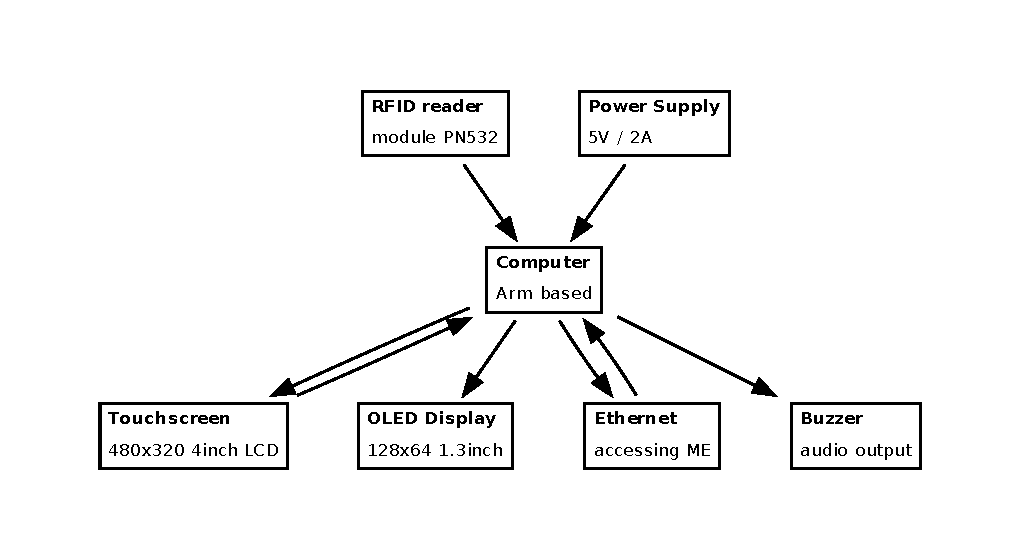
\includegraphics[width=145mm]{../img/hardware}
\caption{Hardware schéma}
\label{hardwareGraph}
\end{figure}

% ORIGNAL TEXT:
% Hardware je založen na mikropočítači, který je osazen procesorem s architekturou typu ARM.
% Z mnoha dnes dostupných ARM počítačů jsem zúžili výběr na následující čtyři:
% Omega 2, NanoPi Neo, Orange Pi Zero a VoCore 2.
% Ty byly vybrány díky své malé velikosti a nainstalovaným ethernet portem,
% který je nezbytný pro připojení do databaze,
% protože jsme nechtěli zvolit připojení do sítě pomocí wifi,
% které je podle našeho názorů nestabilní a nespolehlivé.

% VoCore 2 vyhovoval ve všech bodech, ale byl zamítnut díky vysoké ceně.
% Omega 2 bylo zamítnuto, protože nebyla žádná výhoda oproti konkurenci.
% NanoPi Neo a Orange Pi Zero jsou velmi podobné.
% Nakonec jsme zvolili Orange Pi Zero díky nepatrně lepší výbavě.

% Pro zobrazení pro koncové uživatele jsme vybrali standardní rezistivně dotykový displej o
% rozlišení 480x320 pixelů a průměrem 4 place. Ten komunikuje s počítačem pomocí protokolu SPI,
% aby byla dosažena nízká odezva a plynulost displeje. Tento displej je použit pro obsluhu čtečky.
% Naopak pro strávníky je zde displej s technologií OLED, rozlišením 128x64 pixelů,
% průměrem 1,3 palce, modré barvy. Zde jsou zobrazeny informace určeny pro strávníka.


% Roli samotného čtení čipů nebo mobilů, zajišťuje NFC čtečka založena na
% čipu PN532 a desce 3. verze. Modul čte na frekvenci 13,56 MHz.

% Napájení Orange Pi Zero (Dále už jen OPZ) jsme navrhli pomocí PoE (Power over Ethernet),
% kde OPZ má na své desce rozpojené spojení pro vypnutí této funkce.
% Stačilo tedy jen spojit vývody na desce pomocí cínu.
% Tím se krajní piny ethernet portu propojí s interním regulátorem OPZ.
% Tím se zjednoduší zapojení, ale pokud spojení přesáhne 10 metrů
% začne se snižovat napětí díky vysokému odporu ethernetového drátu,
% což má za následek nedostatečné napájení pro čtečku.

% Při zapojení jsme zjistili, že OPZ obsahuje jen dva přepínací porty SPI,
% což je dostačující pro dotykový displej (obraz a dotyk), ale poté nezbývají
% další SPI piny pro OLED displej ani čtečku, které měly být také připojeny pomocí
% SPI pro dosažení nízké latence. Proto jsme NFC reader přepnuli do protokolu I2C,
% a tím jsme zajistili komunikaci. U displeje byl problém složitější, protože 
% přepínání protokolů je zajištěno odporem mezi spojeními. Pro obavu z poškození
% displeje jsme vyměnili displej za jeho menší verzi (0,96 palce), který má
% nativně podporuje protokol I2C a tím se vyřešily problémy s počtem pinů.

% Počítač byl nahrazen za Raspberry Pi A+ první generace, díky softwarové
% nekompatibilitě grafiky dotykového displeje. Ten nativně neobsahuje ethernetový port,
% a proto byl dodán adaptér z usb na ethernet port, pomocí kterého je zajištěna komunikace
% se serverem a opravnování softwaru přes protokol SSH.
% Upravování kódu je díky tomu možné pouze přes SSH, protože počítač má jen jedno
% usb a bylo by velmi časově náročné provádět úpravy pomocí dotykového displeje.
% \chapter{Software jídelní čtečky}


\chapter{Instalace}

Mocasys je komplexní projekt složený z několika částí, tudíž je instalace
komplikovaný proces zahrnující vícero programovacích jazyků a prostředí.
Momentálně je jediným podporovaným operačním systémem pro vývoj Mocasysu a
spuštění serverových částí GNU/Linux.

Tyto instrukce byly ověřeny na Arch Linuxu a balíčcích z května 2019. Návod
předpokládá, že máte stažené všechny repozitáře projektu ve struktuře složek
určené submoduly.

\section{Instalace Backendu}

\begin{itemize}
    \item Nejprve nainstalujte PostgreSQL \citep[viz][]{PostgreSQL} verze 11 a
    vytvořte prázdné databázové schéma.
    
    \item Stáhněte, zkompilujte a nainstalujte rozšíření PostgreSQL
    temporal\_tables \citep[viz][]{TemporalTables}.

    \item Ve složce \texttt{mocasys-backend} spusťte skript
    \texttt{setup\_db.sh}. Skriptu můžete dát další parametry, které budou
    předány použitému příkazu \texttt{psql}.
\end{itemize}

\section{Instalance Middleendu}

\begin{itemize}
    \item Nainstalujte Node.js \citep[viz][]{NodeJs} a NPM \citep[viz][]{Npm}.

    \item Upravte soubor \texttt{mocasys-middleend/config/default.json} tak,
    aby obsahoval správné nastavení pro připojení k databázi. Middleend využívá
    dvě databázová spojení, \uv{middleend} a \uv{qdb}. \uv{Middleend} by měl
    být připojen pomocí uživatele, který má přístup k tabulkám
    \texttt{user\_passwords\_data} a \texttt{user\_mifare\_cards\_current}.
    \uv{Qdb} používá uživatele \texttt{uptest}, který byl vytvořen skriptem
    \texttt{setup\_db.sh}.

    \item Ve složce \texttt{mocasys-middleend} spusťte příkaz
    \verb|npm install|, což nainstaluje NPM balíčky, a
    \texttt{npm run start}, což spustí server middleendu.
\end{itemize}

\section{Instalace Frontendu}

\begin{itemize}
    \item Nainstalujte SBT \citep[viz][]{Sbt}.

    \item Ve složce \texttt{mocasys-frontend} spusťte příkaz \texttt{sbt
    devel}, poté \texttt{devserver.py}, což spustí webserver hostující
    aplikaci.

    \item Navštivte ve webovém prohlížeči stránku \texttt{http://127.0.0.1:8080}.
\end{itemize}


\chapter*{Závěr}
\addcontentsline{toc}{chapter}{Závěr}

Výsledný soubor programů splňuje zádání kromě hardwarové části, která
se ukázala být problematická. Přestože jsme se rozhodli pro některé
části zvolit vlastní frameworky a knihovny, volba se vyplatila.
Jakmile jsme je totiž měli hotové, vývoj byl velice rychlý.

V budoucnu plánujeme projekt plně dokončit ve všech aspektech a
rozšiřovat ho pro různé typy produkčních provozů


%%% Seznam použité literatury
%%% Seznam použité literatury (bibliografie)
%%%
%%% Pro vytváření bibliografie používáme bibTeX. Ten zpracovává
%%% citace v textu (např. makro \cite{...}) a vyhledává k nim literaturu
%%% v souboru literatura.bib.
%%%
%%% Příkaz \bibliographystyle určuje, jakým stylem budou citovány odkazy
%%% v textu. V závorce je název zvoleného souboru .bst. Styly plainnat
%%% a unsrt jsou standardní součástí latexových distribucí. Styl czplainnat
%%% je dodáván s touto šablonou a bibTeX ho hledá v aktuálním adresáři.

\bibliographystyle{czplainnat}    %% Autor (rok) s českými spojkami
% \bibliographystyle{plainnat}    %% Autor (rok) s anglickými spojkami
% \bibliographystyle{unsrt}       %% [číslo]

\renewcommand{\bibname}{Seznam použité literatury}

%%% Vytvoření seznamu literatury. Pozor, pokud jste necitovali ani jednu
%%% položku, seznam se automaticky vynechá.

\bibliography{literatura}

%%% Kdybyste chtěli bibliografii vytvářet ručně (bez bibTeXu), lze to udělat
%%% následovně. V takovém případě se řiďte normou ISO 690 a zvyklostmi v oboru.

% \begin{thebibliography}{99}
%
% \bibitem{lamport94}
%   {\sc Lamport,} Leslie.
%   \emph{\LaTeX: A Document Preparation System}.
%   2. vydání.
%   Massachusetts: Addison Wesley, 1994.
%   ISBN 0-201-52983-1.
%
% \end{thebibliography}


%%% Obrázky v bakalářské práci
%%% (pokud jich je malé množství, obvykle není třeba seznam uvádět)
\listoffigures

%%% Tabulky v bakalářské práci (opět nemusí být nutné uvádět)
%%% U matematických prací může být lepší přemístit seznam tabulek na začátek práce.
\listoftables

%%% Použité zkratky v bakalářské práci (opět nemusí být nutné uvádět)
%%% U matematických prací může být lepší přemístit seznam zkratek na začátek práce.
% \chapwithtoc{Seznam použitých zkratek}

%%% Přílohy k bakalářské práci, existují-li. Každá příloha musí být alespoň jednou
%%% odkazována z vlastního textu práce. Přílohy se číslují.
%%%
%%% Do tištěné verze se spíše hodí přílohy, které lze číst a prohlížet (dodatečné
%%% tabulky a grafy, různé textové doplňky, ukázky výstupů z počítačových programů,
%%% apod.). Do elektronické verze se hodí přílohy, které budou spíše používány
%%% v elektronické podobě než čteny (zdrojové kódy programů, datové soubory,
%%% interaktivní grafy apod.). Elektronické přílohy se nahrávají do SISu a lze
%%% je také do práce vložit na CD/DVD. Povolené formáty souborů specifikuje
%%% opatření rektora č. 72/2017.
% \appendix
% \chapter{Přílohy}

% \openright
\end{document}
